\documentclass[aspectratio=43]{beamer}
% \documentclass[aspectratio=43]{beamer}
% ---------------------------
% Set the aspectration variable before!
% ---------------------------
\newcommand{\myaspectratio}{43} % <-- set to 43 or 169

% ---------------------------
% Custom colors
% ---------------------------
\definecolor{mainblue}{RGB}{100,149,237}
\definecolor{ghostwhite}{RGB}{242,244,245}

% ---------------------------
% Font (XeLaTeX or LuaLaTeX required)
% ---------------------------
%\usepackage{fontspec}
% Configure your custom font
% \setsansfont{AlanSans.ttf}[
%   Path=./AlanSansFont/,                      % Path to the folder containing your font files
%   Extension=.ttf,               % Specify the font file extension
%   UprightFont=*-UpRight.ttf,    % Link the regular font file
%   BoldFont=*-Regular.ttf           % Link the bold font file
%   % ItalicFont=*-Italic.ttf
% ]

% ---------------------------
% Emoji
% ---------------------------
% \usepackage{emoji} % LuaLatex
% \usepackage{twemojis} % XeLatex

% ---------------------------
% Social icons
% ---------------------------
% \usepackage{fontawesome5} 

% ---------------------------
% Minimal Beamer theme
% ---------------------------
\usetheme{default}
\setbeamercolor{normal text}{fg=black,bg=ghostwhite}
\setbeamercolor{structure}{fg=mainblue}
\setbeamercolor{frametitle}{fg=white,bg=}

% Move frametitle slightly down
\setbeamertemplate{frametitle}{%
  \vspace{0.5cm} % <-- adjust this value
  \nointerlineskip%
  \begin{beamercolorbox}[wd=\paperwidth,sep=0.3cm,left]{frametitle}%
  \usebeamerfont{frametitle}\insertframetitle
  \end{beamercolorbox}%
}


% Remove navigation symbols
\setbeamertemplate{navigation symbols}{}

% ---------------------------
% Packages
% ---------------------------
\usepackage{graphicx}
\usepackage{amsmath}
\usepackage{multicol}

% ---------------------------
% Aspect ratio selector
% ---------------------------

\newcommand{\choosebackground}{%
  \ifnum\myaspectratio=43
    \def\mybackground{background_43.png}%
  \else
    \ifnum\myaspectratio=169
      \def\mybackground{background_169.png}%
    \else
      \def\mybackground{background.png}% fallback
    \fi
  \fi
}
\choosebackground

\setbeamertemplate{background canvas}{%
  \includegraphics[width=\paperwidth]{\mybackground}%
}

% ---------------------------
% Title slide (no background, no numbering)
% ---------------------------
% usa se non hai ancora il pacchetto per i loghi social
% \usepackage{fontawesome5} 

\newcommand{\plainTitlePage}[2]{% #1 = immagine grande, #2 = lista social
  {%
    % background ghostwhite
    \setbeamertemplate{background canvas}[vertical shading][bottom=ghostwhite,top=ghostwhite]

    \begin{frame}[plain] % plain = no footer
      \vfill
      \begin{columns}[T,totalwidth=\textwidth]
        % Text column
        \column{0.6\textwidth}
          \raggedleft
          {\color{mainblue}\Huge \inserttitle\par}
          \bigskip\bigskip
          {\Large \insertauthor\par}
          \medskip
          {\large \insertdate\par}

          % Social links area
          \raggedleft
          {\small #2}

        % Space between columns
        \hspace{1cm}

        % Image column
        \column{0.35\textwidth}
          \centering
          \includegraphics[width=\linewidth]{#1}
      \end{columns}
      \vfill
    \end{frame}

    % restore background afterwards
    \setbeamertemplate{background canvas}{%
      \includegraphics[width=\paperwidth]{\mybackground}%
    }
  }%
}


% ---------------------------
% Frame numbering in bottom-right corner
% ---------------------------
\setbeamertemplate{footline}{%
  \leavevmode%
  \hfill%
  \usebeamerfont{footline}\usebeamercolor[fg]{footline}%
  {\tiny \insertframenumber{} / \inserttotalframenumber}%
  \hspace{0.5cm}\vspace{0.2cm}%
}
\setbeamerfont{footline}{size=\small}

% ---------------------------
% Document info
% ---------------------------
\title{NotebookLM en la Enseñanza de la Ingeniería Eléctrica (CMI)}
\author{Dr. Vladímir Rodríguez Diez}
\date{\today}

\begin{document}
% Cheatsheet: https://www.ipgp.fr/~moguilny/LaTeX/fontawesome5Icons.pdf
\plainTitlePage{Gemini_Generated_Image_btmeajbtmeajbtme.png}{%
  % \faTwitter\ \href{https://twitter.com/vladimir12}{@myuser}\\
   % \faGithub\ \href{https://github.com/vladimir1284}{github.com/vladimir1284}\\
   % \faLinkedin\ \href{https://linkedin.com/in/vladímir-rodríguez-diez-12a76649}{/in/vladímir-rodríguez-diez}%
}

\begin{frame}
\frametitle{Potenciando la Enseñanza de la Ingeniería Eléctrica con Google NotebookLM}
\begin{itemize}
    \item \textbf{Tipo de Actividad:} \textbf{Clase Metodológica Instructiva (CMI)}.
    \item \textbf{Función:} Orientar e \textbf{instruir} a los docentes de la disciplina de Accionamientos Eléctricos mediante la \textbf{argumentación y el análisis}.
    \item \textbf{Finalidad:} Elevar la \textbf{maestría pedagógica} del colectivo de disciplina y la calidad del proceso docente-educativo (PDE).
\end{itemize}
\end{frame}

\begin{frame}
\frametitle{ChatGPT responde a una pregunta de clases}
\begin{center}
  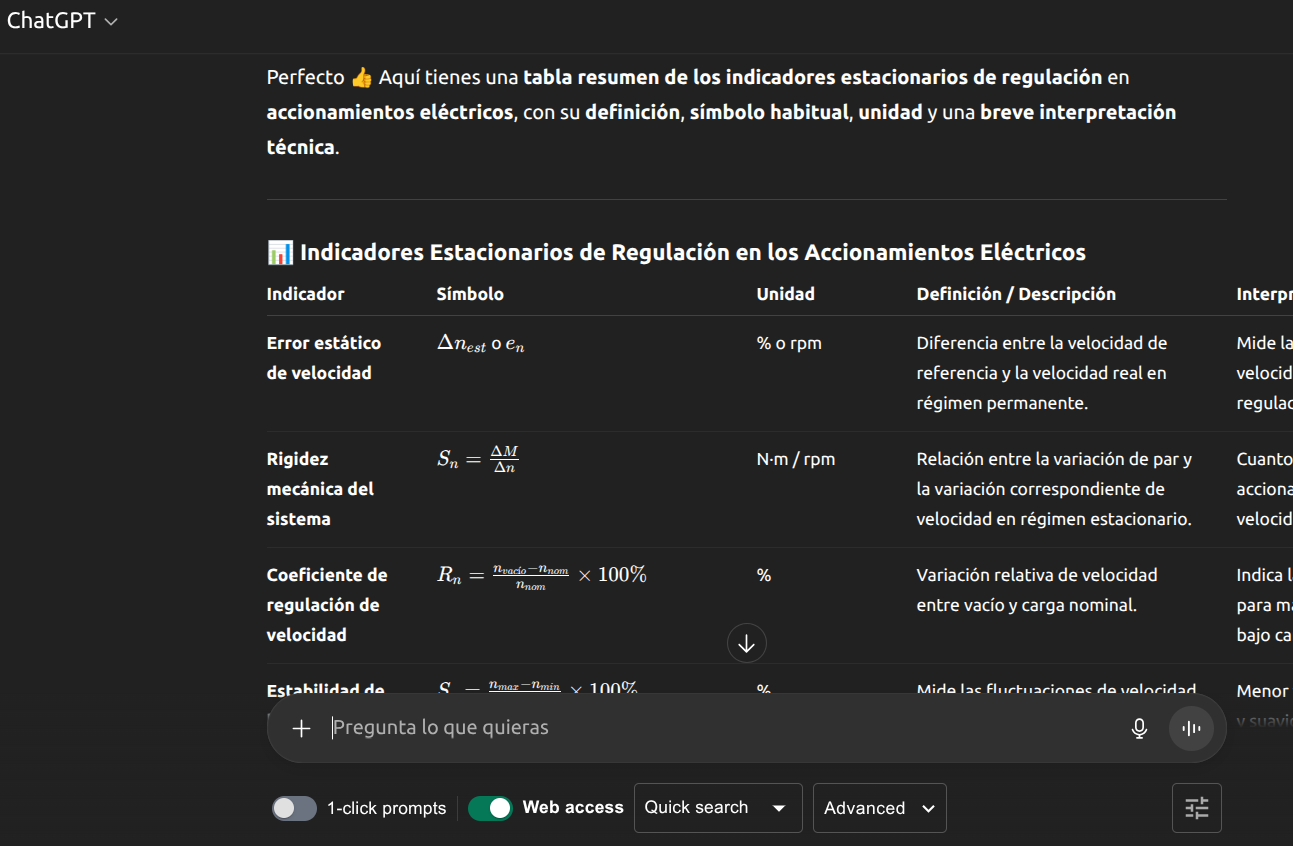
\includegraphics[width=3.5in]{chat_gpt.png}
\end{center}
\end{frame}

\begin{frame}
\frametitle{El Problema Conceptual Metodológico}

\textbf{El Problema (La Contradicción Didáctica):}
\begin{itemize}
    \item Las IAs generativas convencionales (LLMs) presentan un riesgo alto de \textbf{alucinación} (información inexacta o fabricada).
    \item Esto es crítico en Ingeniería Eléctrica (EE), donde el \textbf{rigor científico-técnico} y la \textbf{precisión} son insustituibles.
    \item Se necesita una solución que permita la \textbf{innovación pedagógica} sin sacrificar la \textbf{integridad académica}.
\end{itemize}

\vfill

\textbf{Planteamiento:}
\begin{quote}
¿Cómo integrar eficazmente la IA para \textbf{diseñar recursos didácticos especializados}, garantizando su \textbf{coherencia curricular} y el \textbf{rigor técnico}, y superando la falta de contextualización de las IAs genéricas?
\end{quote}
\end{frame}

\begin{frame}
\frametitle{Objetivo Metodológico y Estrategia}

\textbf{Objetivo Metodológico (El \textit{Para Qué})}:
\begin{quote}
\textbf{Instruir} a los docentes en el uso de \textbf{NotebookLM (NLM)} como un \textbf{Asistente de Cátedra especializado}, fundamentado en la \textbf{bibliografía de autoridad} seleccionada por el profesor, para perfeccionar la \textbf{preparación didáctica} y la creación de contenidos en la enseñanza de la Ingeniería Eléctrica.
\end{quote}
\vfill
\textbf{Estrategia Metodológica}:
\begin{itemize}
  {\small
    \item Esta CMI (\textit{Instructiva}) se inserta en un sistema de trabajo docente-metodológico.
    \item Será seguida de una Clase Abierta o una Clase Demostrativa (CMD) para comprobar la apropiación colectiva del "cómo hacerlo".
  }
  \end{itemize}
\end{frame}

\begin{frame}
\frametitle{Sumario (Plan de la CMI)}

\textbf{I. Introducción:} Problema y Objetivo Metodológico.

\textbf{II. Desarrollo: El Cómo} (Análisis y Argumentación)
\begin{enumerate}
    \item Fundamentos de NLM: Arquitectura \textbf{Grounded AI} / RAG.
    \item Aplicaciones Estratégicas en EE (Diseño, Aula, Investigación, Evaluación).
    \item Argumentación Metodológica y Debate.
\end{enumerate}

\textbf{III. Conclusiones:} Síntesis, Recomendaciones y Aspectos Éticos.
\end{frame}

\begin{frame}
\frametitle{Introducción a NotebookLM}

\textbf{NLM:} Herramienta de IA diseñada para \textbf{análisis avanzado de documentos} y \textbf{generación de contenido educativo}.

\vfill
\textbf{Características Clave para la Educación Superior:}
\begin{itemize}
    \item \textbf{Fuentes Propias (RAG):} Interactúa con documentos subidos por el usuario (PDFs, transcripciones, Google Docs/Slides).
    \item \textbf{Privacidad:} Google no utiliza los datos personales, subidas o consultas para entrenar el modelo (excepto para usuarios menores de 18, con políticas más estrictas).
    \item \textbf{Citación Transparente:} Todas las respuestas incluyen \textbf{citas} en línea que remiten a las fuentes originales, fomentando la \textbf{integridad académica}.
\end{itemize}
\end{frame}

\begin{frame}
\frametitle{Fundamento Metodológico: RAG y el Rigor Técnico}

\textbf{Arquitectura RAG (Retrieval-Augmented Generation)}:
\begin{itemize}
    \item El sistema basa sus salidas \textbf{exclusivamente} en la información extraída de los documentos fuente cargados por el usuario.
    \item Esto \textbf{minimiza el riesgo de alucinación} (información fabricada), un problema crucial en temas de Ingeniería Eléctrica.
\end{itemize}
\vfill
\textbf{El Valor NLM en EE (Tesis Central)}:
\begin{quote}
NLM se convierte en un \textbf{experto instantáneo} sobre \textbf{nuestra} bibliografía. Proporciona \textbf{Especialización sobre Fuentes Confiables}, ya sean normas, manuales técnicos o apuntes de cátedra.
\end{quote}
\end{frame}



\begin{frame}
  \frametitle{NLM responde a la misma pregunta de clases}
  \begin{center}
    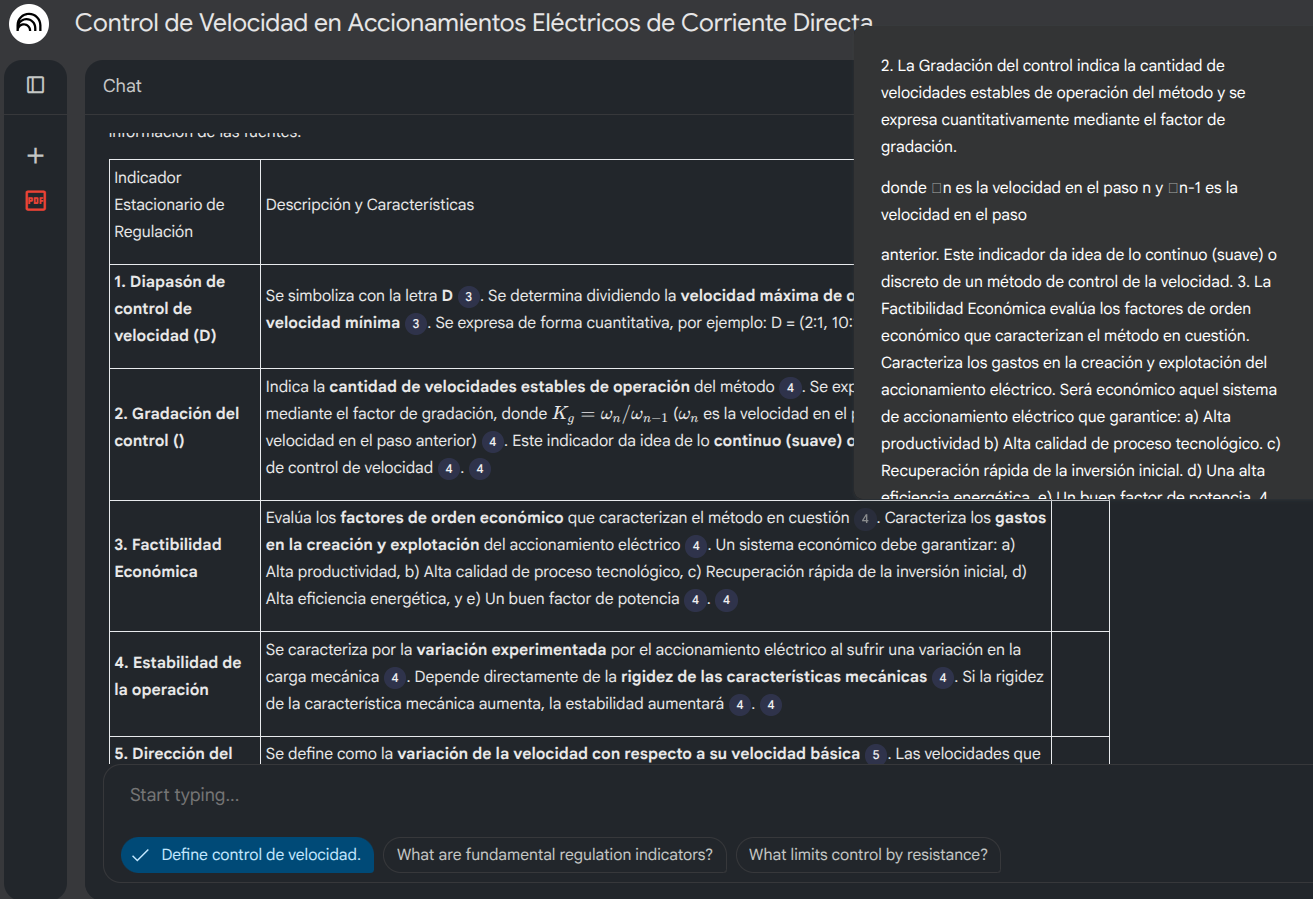
\includegraphics[width=3.5in]{indicadores.png}
  \end{center}
  \end{frame}

\begin{frame}
\frametitle{Tipos de Fuentes Técnicas Soportadas}

\textbf{NLM acepta una variedad de formatos esenciales para EE}:
\begin{itemize}
    \item \textbf{Documentos:} Archivos PDF (manuales de equipos, hojas de datos, normativas: NEC, IEC, IEEE).
    \item \textbf{Material de Curso:} Google Docs/Slides, apuntes del profesor (para asegurar la alineación de la enseñanza).
    \item \textbf{Contenido Digital:} Sitios web (enlaces) y transcripciones de videos de YouTube (copiar/pegar texto).
\end{itemize}
% \vfill
% \textbf{Consideración Metodológica Importante:}
% \begin{itemize}  
%     \item \textbf{Símbolos Matemáticos:} {\small Algunos símbolos pueden \textbf{no mostrarse correctamente} en la salida inicial. Se recomienda usar NLM para el texto base y luego herramientas como Google Gemini para corregir y renderizar los símbolos correctamente.}
% \end{itemize}
\end{frame}

% \begin{frame}
% \frametitle{Limitaciones y Precauciones Éticas}

% \textbf{Desafíos Metodológicos y Técnicos}:
%   \begin{itemize}
%       \item \textbf{Riesgo de Sobre-Confianza:} Los documentos cargados pueden contener \textbf{errores o información desactualizada}. NLM solo es tan bueno como sus fuentes.
%       \item \textbf{Supervisión Docente:} El profesor es imprescindible para asegurar la \textbf{precisión pedagógica}.
%       \item \textbf{Equidad y Costo:} Existe una versión \textit{Plus} (de pago), lo que plantea preocupaciones sobre la \textbf{equidad y el acceso} para estudiantes o instituciones con menos recursos.
%   \end{itemize}
% \end{frame}

% \begin{frame}
%   \frametitle{Limitaciones y Precauciones Éticas}
%   \textbf{Desafíos Metodológicos y Técnicos}:
%   \begin{itemize}
%       \item \textbf{Propiedad Intelectual (IP):} Compartir \textit{notebooks} con material protegido por derechos de autor (ej. artículos de revistas) puede infringir la ley de copyright, a menos que el usuario tenga plenos derechos o se comparta en modo "solo chat".
%       \item \textbf{Riesgo Institucional:} Precedentes de Google de discontinuar servicios (ej. Google Jamboard) crean incertidumbre sobre la \textbf{disponibilidad a largo plazo}.
%   \end{itemize}
% \end{frame}


% II.B. Aplicaciones Estratégicas en Ingeniería Eléctrica

\begin{frame}
\frametitle{Aplicación A: Preparación y Diseño Instruccional}

\textbf{1. Creación de Bancos de Preguntas Avanzados}:
\begin{itemize}
    \item Cargar el \textbf{programa de la asignatura} y \textbf{normativas técnicas} (NEC, IEC).
    \item Solicitar preguntas de examen que se alineen \textbf{estrictamente} con las fuentes cargadas.
\end{itemize}

\textbf{2. Desarrollo de Guías de Laboratorio Seguras}:
\begin{itemize}
    \item Subir \textbf{manuales de equipos} (e.g., transformadores, relés) y \textbf{protocolos de seguridad}.
    \item Pedir a NLM que \textbf{verifique y refine la guía}, cruzando procedimientos con advertencias de fabricantes, mitigando riesgos.
\end{itemize}
\end{frame}

\begin{frame}
  \frametitle{Pregunta para examen}
  \begin{center}
    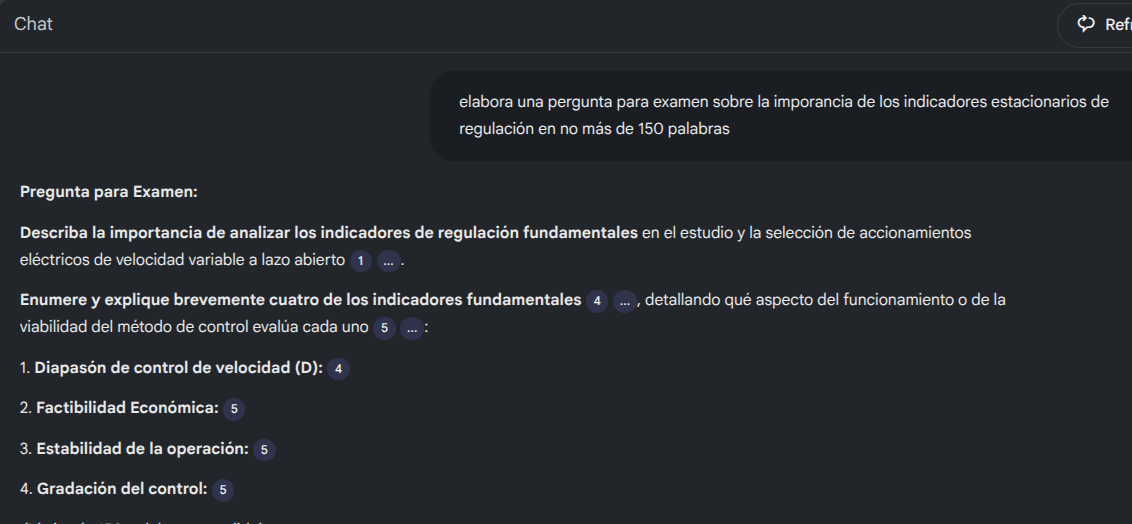
\includegraphics[width=4.5in]{pregunta.png}
  \end{center}
\end{frame}

\begin{frame}
\frametitle{ Aplicación B: Ejecución en el Aula y Aprendizaje Activo}

\textbf{3. Simulador de "El Experto en la Sala"}:
\begin{itemize}
    \item Cargar notas de clase y \textit{papers} especializados.
    \item Estudiantes preguntan sobre conceptos técnicos complejos; NLM actúa como un experto que solo conoce esa bibliografía, fomentando \textbf{preguntas profundas}.
\end{itemize}

\textbf{4. Análisis Crítico de Normativas (IE/EE)}:
\begin{itemize}
    \item Cargar un nuevo \textit{paper} y una \textbf{normativa IEEE}.
    \item Estudiantes usan NLM para \textbf{identificar puntos clave} y verificar el \textbf{cumplimiento normativo} del artículo.
\end{itemize}
\end{frame}

\begin{frame}
\frametitle{ Aplicación B: Resolución Guiada de Problemas}

\textbf{5. Resolución Guiada de Problemas Complejos (\textit{Scaffolding})}:
\begin{itemize}
    \item Cargar \textbf{problemas resueltos} por el profesor y la \textbf{metodología de solución}.
    \item El estudiante pregunta: “Basándote en los ejercicios, ¿cuál es el primer paso para abordar este nuevo problema de control?”.
    \item \textbf{Valor Metodológico:} Proporciona ayuda \textbf{contextualizada} que guía la metodología sin entregar la solución final, apoyando el \textbf{diálogo socrático} y el \textbf{aprendizaje activo}.
\end{itemize}
\end{frame}

\begin{frame}
  \frametitle{Resolución Guiada de Problemas Complejos}
  \begin{center}
    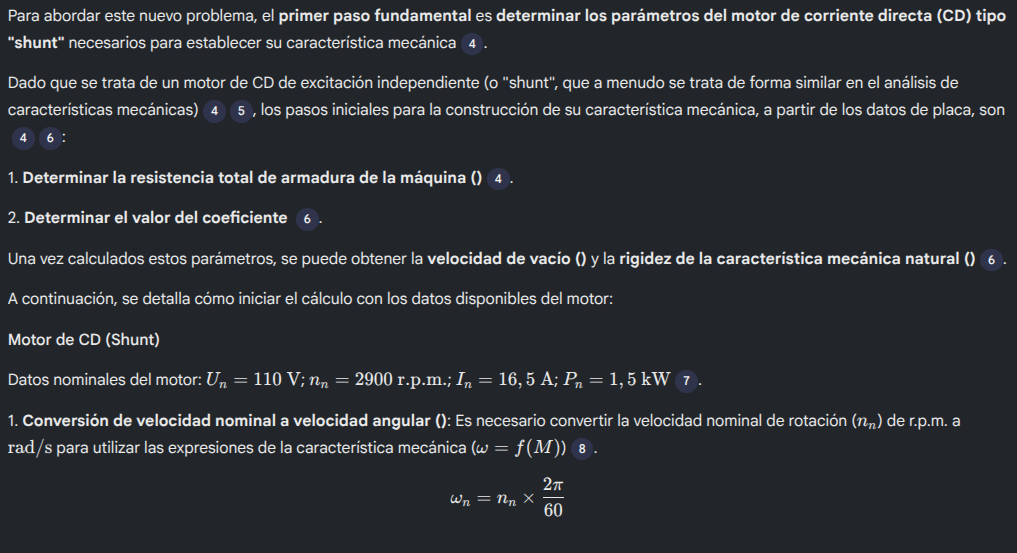
\includegraphics[width=4in]{solucion.png}
  \end{center}
\end{frame}

\begin{frame}
\frametitle{ Aplicación C: Multimodalidad y Neurodiversidad}

\textbf{NLM soporta salidas multimodales para diversas preferencias cognitivas}:
\begin{itemize}
    \item \textbf{Mind Maps:} Analiza las fuentes y crea mapas mentales para \textbf{visualizar cómo los temas están interconectados} (Ej. conceptos de Electrónica de Potencia).
    \item \textbf{Video Overviews:} Genera un video con \textbf{voz en off y diapositivas} para resumir el contenido (útil para el repaso rápido).
    \item \textbf{Audio Overviews/Podcasts:} Convierte textos densos (ej. sobre controladores PID) en \textbf{diálogos conversacionales} entre dos agentes de IA.
\end{itemize}
\end{frame}

\begin{frame}
  \frametitle{Mapa Conceptual}
  \begin{left}
    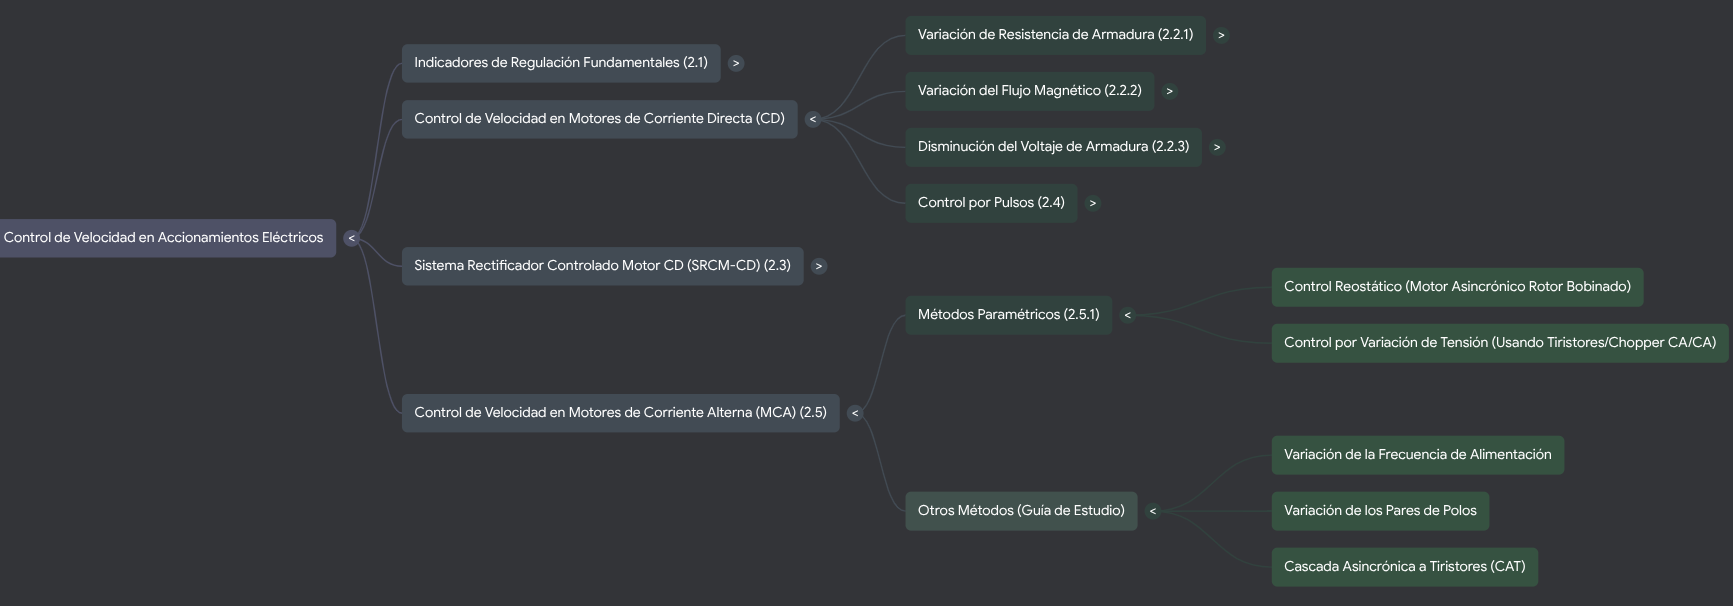
\includegraphics[width=4.3in]{mindmap.png}
  \end{left}
\end{frame}

\begin{frame}
\frametitle{ Aplicación C: Multimodalidad y Neurodiversidad}

\textbf{Modo Interactivo (Interactive Mode)}:
\begin{itemize}
    \item El estudiante puede \textbf{unirse al podcast en tiempo real} y hacer preguntas a los agentes, extendiendo la discusión dinámicamente.
\end{itemize}
\end{frame}

\begin{frame}
\frametitle{ Aplicación D: Tutoría Personalizada}

\textbf{6. Creación de Tutores de Materia Personalizados (24/7)}:
\begin{itemize}
    \item El docente crea y comparte un \textbf{notebook por unidad} con apuntes, presentaciones y lecturas obligatorias.
    \item El estudiante interactúa con un \textbf{asistente AI} que responde \textbf{exclusivamente} con la \textbf{terminología y consistencia} del curso.
\end{itemize}

\textbf{7. Tutoría Adaptativa Basada en Desempeño}:
\begin{itemize}
    \item Cargar \textbf{informes de evaluación} del estudiante.
    \item Pedir a NLM que sugiera un \textbf{plan de repaso} enfocado en las competencias de EE menos desarrolladas, utilizando capítulos específicos del libro de texto cargado.
\end{itemize}
\end{frame}

\begin{frame}
\frametitle{ Aplicación D: Evaluación Asistida y Rigurosa}

\textbf{8. Evaluación Automática Asistida por Criterios}:
\begin{itemize}
    \item El docente carga la \textbf{rúbrica oficial} y la \textbf{tarea entregada por el estudiante}.
    \item NLM genera un informe de evaluación (fortalezas/debilidades) basado \textbf{solo en los criterios definidos} en la rúbrica.
    \item \textbf{Beneficio:} Automatiza la retroalimentación, mejora la \textbf{consistencia evaluativa} y fomenta la \textbf{alfabetización en evaluación} (\textit{assessment literacy}).
\end{itemize}

\end{frame}

\begin{frame}
\frametitle{ Aplicación E: Investigación Académica y Desarrollo}
\textbf{9. Guía de Preparación para Exámenes}:
\begin{itemize}
    \item Subir \textbf{transcripciones de clases} y \textbf{cuestionarios de años anteriores}.
    \item NLM puede generar \textbf{guías de estudio}, \textbf{FAQs}, y resúmenes temáticos.
\end{itemize}

\textbf{NLM como Compañero de Investigación y Síntesis}:
\begin{itemize}
    \item \textbf{Revisión de Literatura (Tesis de Grado):} Cargar múltiples \textit{papers} (ej. sobre energías renovables).
    \item NLM sintetiza el \textbf{estado del arte}, identifica \textbf{puntos en común y contradicciones} entre autores, y señala \textbf{vacíos de investigación}.
\end{itemize}
\end{frame}

\begin{frame}
  \frametitle{ Aplicación E: Investigación Académica y Desarrollo}
\textbf{10. Análisis y Síntesis de Documentos Técnicos Densos}:
\begin{itemize}
    \item Cargar la \textbf{hoja de datos} de un componente y el \textbf{manual} de un equipo.
    \item Preguntar a NLM que \textbf{conecte información de ambos documentos} para resolver una duda aplicada (ej. conectar un MOSFET a un microcontrolador).
\end{itemize}
\end{frame}

\begin{frame}
\frametitle{ Aplicación E: Gestión Curricular e Institucional}

\textbf{11. Revisión y Unificación Curricular:} 
\begin{itemize}
    \item Cargar \textbf{programas de asignaturas correlativas} (Ej. Circuitos I, II, Máquinas).
    \item Pedir a NLM que \textbf{identifique redundancias, vacíos temáticos o inconsistencias} entre los contenidos para mejorar la coordinación curricular.
\end{itemize}

\vfill
\textbf{12. Acreditación Académica}:
\begin{itemize}
    \item Cargar los \textbf{criterios del ente acreditador} (ABET, etc.) y los \textbf{resultados de aprendizaje}.
    \item NLM genera un \textbf{resumen del cumplimiento} de los criterios, acelerando la autoevaluación institucional.
\end{itemize}
\end{frame}

\begin{frame}
\frametitle{ Aplicación F: Uso del Estudio (Studio) para Recursos}

\textbf{El Studio: Generación Rápida de Recursos}:
\begin{itemize}
    \item Permite generar automáticamente, a partir de las fuentes cargadas:
    \item \textbf{Flashcards} y \textbf{Quizzes} (preguntas de opción múltiple).
    \item \textbf{Reportes} (Study Guide, FAQ, Briefing Doc, Timeline).
    \item \textbf{Mind Maps} (para desglosar conceptos y temas).
\end{itemize}

\vfill
\textbf{Uso en Cátedra}:
\begin{itemize}
    \item Los quizzes generados pueden ser \textbf{renombrados} (ej. Quiz A, Quiz B) y \textbf{compartidos} con los estudiantes mediante email o enlace web.
\end{itemize}
\end{frame}

% II.C. Argumentación Didáctica y Metodológica

\begin{frame}
\frametitle{ La Integración NLM y Pedagogía Constructivista}

\textbf{Argumentación Didáctica:}
\begin{itemize}
    \item NLM facilita la \textbf{interacción dialéctica con el material}.
    \item Promueve la \textbf{alfabetización en IA (GenAI Literacy)}: Enseña a evaluar, usar éticamente y criticar las salidas de IA.
    \item Apoya la \textbf{autorregulación del aprendizaje}, ya que los estudiantes se hacen cargo de la planificación, el monitoreo y la evaluación de su estudio.
\end{itemize}
\vfill
\textbf{El Rol del Docente de EE}:
\begin{itemize}
    \item El profesor no es un generador de \textit{prompts}, sino un \textbf{curador de fuentes de autoridad} y un \textbf{validador final} de la precisión pedagógica.
\end{itemize}
\end{frame}

%III. Conclusiones (Diapositivas 21-25)

\begin{frame}
\frametitle{ Valoración del Cumplimiento del Objetivo Metodológico }

\begin{itemize}
    \item Se logró instruir a los docentes al demostrar que NLM, gracias a su \textbf{arquitectura RAG}, proporciona una vía para la \textbf{innovación pedagógica} sin comprometer el \textbf{rigor técnico}.
\end{itemize}

\textbf{Síntesis y Consolidación}:
\begin{itemize}
    \item NLM es una herramienta \textbf{grounded, flexible y consciente del contexto}.
    \item Actúa como un \textbf{co-diseñador pedagógico} que acelera la producción de \textbf{material didáctico preciso} (quizzes, guías, tutores), basado en la autoridad del docente.
    \item Promueve la \textbf{evaluación consistente} al fundamentar la retroalimentación en rúbricas oficiales (Assessment Literacy).
\end{itemize}
\end{frame}

\begin{frame}
\frametitle{ Recomendaciones Metodológicas}

\textbf{Orientaciones de Valor Generalizador para el Colectivo}:
\begin{enumerate}
    \item \textbf{Carga de Fuentes Críticas:} Priorizar la carga de \textbf{normativas (IEEE, NEC)} y \textbf{manuales de equipos} para asegurar la contextualización específica de la Ingeniería Eléctrica.
    \item \textbf{Ética y Transparencia:} Instruir a los estudiantes en la verificación constante de las \textbf{citas} que ofrece NLM (función RAG) y utilizar la herramienta para \textbf{síntesis} y \textbf{análisis}, no para la simple generación de contenidos.
    \item \textbf{Aprovechar la Multimodalidad:} Usar \textbf{Audio y Video Overviews} para el repaso de contenidos complejos, beneficiando a estudiantes con preferencias auditivas.
\end{enumerate}
\end{frame}

% \begin{frame}
% \frametitle{ Vínculo con el Trabajo Metodológico Futuro}

% \textbf{La CMI en el Sistema de Trabajo Docente-Metodológico:}
% \begin{itemize}
%     \item La \textbf{Clase Metodológica Instructiva} orientó el \textit{qué} y el \textit{cómo} a nivel conceptual y didáctico.
%     \item Próximo paso: \textbf{Clase Abierta o Demostrativa (CMD)}.
%     \item \textbf{Objetivo de la CMD Sugerida:} Demostrar la aplicación práctica de NLM en una clase de "Análisis de Circuitos" para generar ejercicios y tutores contextualizados, verificando si se ha \textbf{perfeccionado la actuación profesoral}.
% \end{itemize}
% \vfill
% \textbf{Recordatorio:} El \textbf{trabajo metodológico} es esencial para elevar la \textbf{maestría pedagógica} de los docentes y la eficiencia del PDE.
% \end{frame}

% \begin{frame}
% \frametitle{ Evaluación y Actualización Científica}

% \textbf{Aspectos Clave para Evaluar una CMI}:
% \begin{itemize}
%     \item \textbf{Cumplimiento del Objetivo Metodológico} y la estructura de la clase.
%     \item \textbf{Pertinencia} del Problema Conceptual Metodológico.
%     \item \textbf{Rigor} en el abordaje de los aspectos científicos y metodológicos.
%     \item \textbf{Nivel de Actualización} demostrado.
%     \item Calidad y conducción del \textbf{debate}.
% \end{itemize}
% \end{frame}

% \begin{frame}
% \frametitle{ Evaluación y Actualización Científica}

% \textbf{Actualización Constante:}
% \begin{itemize}
%     \item El profesor responsable debe demostrar un \textbf{gran nivel de actualización científica y metodológica}. La integración de herramientas como NLM, que están en constante desarrollo, subraya esta necesidad.
% \end{itemize}
% \end{frame}

\begin{frame}
  \frametitle{ Referencias Bibliográficas}
  
  \textbf{Trabajo Docente Metodológico (CMI y CMD)}
  \begin{enumerate}
      \item MES (2018). Resolución 2/2018 (Reglamento). Tipos de trabajo docente-metodológico.
      \item Moral Roldan, J. (s.f.). Clase Metodológica. Planificación, introducción, desarrollo y conclusiones.
      \item Anónimo (s.f.). Clase Metodológica (EcuRed). Concepto y organización escalonada (reunión, clase, control).
      \item Barazal y Expósito (2010). Clase Metodológica en ES. Estrategia para elevar la maestría pedagógica.
  \end{enumerate}
\end{frame}

\begin{frame}
  \frametitle{ Referencias Bibliográficas}
  \begin{enumerate}
      \item Machado Díaz et al. (2023). Manual CMI. Estructura de la CMI; problema conceptual metodológico como centro de la clase.
      \item Batista Salvador et al. (s.f.). Fundamentos CMI/CMD. Guía metodológica y didáctica; alternativas de estructura para la CMI.
  \end{enumerate}
  
  \textbf{Google NotebookLM: Características y Usos Generales}
  \begin{enumerate}    
    \item Reyna, J. (2025). Potencial de NotebookLM. Rol en investigación, estudio y docencia; arquitectura RAG para reducir alucinación.
  \end{enumerate}
\end{frame}

\begin{frame}
  \frametitle{ Referencias Bibliográficas}

  \begin{enumerate}    
    \item Ditch That Textbook (2025). 10 Cosas NLM. Funcionalidades clave (audio/video overviews, mapas mentales, reportes) y gratuidad.
    \item Classnotes Nicole (s.f.). 10 Usos NLM. Creación de recursos como flashcards, cuestionarios, planes de unidad y resúmenes de audio interactivos (podcast).
    \item Huffman y Hutson (2024). NLM en Historia. Estudio de caso para generar contenido multimedia y podcast a partir de un diario.
  \end{enumerate}
\end{frame}

\begin{frame}
  \frametitle{ Referencias Bibliográficas}
  
  \textbf{Google NotebookLM: Aplicaciones Especializadas}
  \begin{enumerate}
      \item CM Ing. Eléctrica (s.f.). NLM en Ingeniería. Aplicación especializada en diseño de bancos de preguntas técnicos, guías de laboratorio y "Tutores de Materia Personalizados".
      \item Saunders y Varga-Atkins (s.f.). NLM y Assessment Literacy. Uso de NLM para generar podcast a partir de descripciones de tareas formativas y assessment briefs para mejorar la comprensión de la evaluación.
  \end{enumerate}
\end{frame}

\begin{frame}
\frametitle{ Preguntas y Comentarios }
\begin{itemize}
    \item Agradecemos su participación activa en esta \textbf{Clase Metodológica Instructiva}.
    \item Abrimos el espacio para un intercambio final sobre las posibles vías para aplicar NLM en sus respectivas asignaturas de Ingeniería Eléctrica.
    \item Recomendaciones para una futura \textbf{Clase Metodológica Demostrativa}
\end{itemize}
\end{frame}

\end{document}
